\documentclass[compress=true]{beamer}
\usepackage{caption}
%\usepackage{xeCJK}
%\setCJKmainfont{WenQuanYi Zen Hei}
\usetheme{Warsaw}
\title{Field regions and power pattens of an antenna}
\author{\tiny{Yimian Dai,Wenbo Wang,Yu Qin,Haiyang Zhang}}
\institute{http://dspandlinux.com}
\begin{document}
% frame_01
\begin{frame}
\titlepage
\end{frame}
% frame_
\begin{frame}
  \frametitle{Outline}
  \begin{block}{\bf E}
    $$E_r = \eta\frac{I_0l\cos{\theta}}{2\pi r^2}[1+\frac{1}{jkr}]e^{-jkr}$$
    $$E_{\theta} = j\eta\frac{kI_0l\sin{\theta}}{4\pi r}[1+\frac{1}{jkr}-\frac{1}{(kr)^2}]e^{-jkr}$$
    $$E_{\phi}=0$$
  \end{block}
  \begin{block}{\bf H}
    $$H_r=H_{\theta}=0$$
    $$H_{\phi}=j\frac{kI_0l\sin{\theta}}{4\pi r}[1+\frac{1}{jkr}]e^{-jkr}$$
  \end{block}
\end{frame}
% frame_
\begin{frame}
  \frametitle{Antenna radiation zoning}
  \begin{itemize}
    \item Near-Field (kr$\ll$1) Region
    \item Intermediate-Field (kr$>$1) Region
    \item Far-Field (kr$\gg$1)
  \end{itemize}
\end{frame}

%% Near
% frame_
\begin{frame}
  \frametitle{Near-Field Region}
\begin{block}{~}
  \begin{equation}
    \left.
      \begin{array}{l}
        E_r \simeq -j{\eta}\frac{I_0le^{-jkr}}{2\pi kr^3}\cos{\theta}\\\\
        E_{\theta} \simeq -j{\eta}\frac{I_0le^{-jkr}}{1\pi kr^3}\sin{\theta}\\\\
        E_{\phi}=H_r=H_{\theta}=0\\\\
        H_{\phi}\simeq \frac{I_0le^{-jkr}}{4\pi r^2}\sin{\theta}
      \end{array}
    \right\}~~~~ kr\ll 1
  \end{equation}
\end{block}
\begin{center}
if~~$f=0.70GHz,kr=0.1$,then\\
$k=\frac{2\pi}{\lambda}=\frac{2\pi f}{c}\simeq 109.4$\\
so~$r=0.000477 m$
\end{center}
\end{frame}
% frame_
\begin{frame}
  \frametitle{Patten of Near-Field Region}
%  \framesubtitle{kr=0.01}
  \begin{figure}
    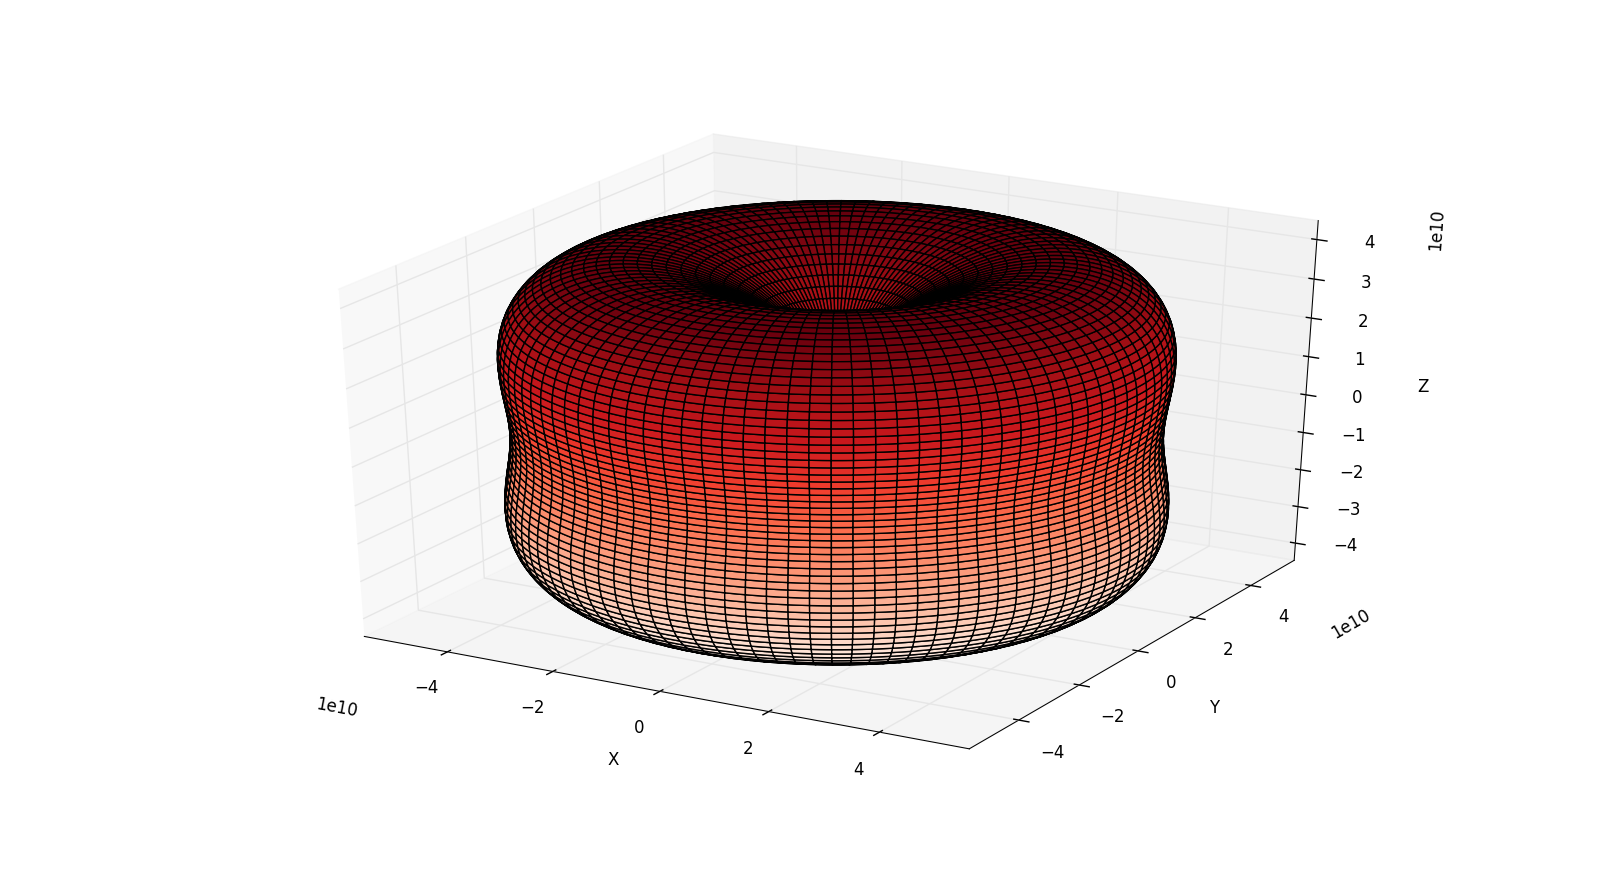
\includegraphics[height=0.7\textheight]{near_kr_0_01_1.png}
    \caption*{\tiny{kr=0.01}}
  \end{figure}
\end{frame}
% frame_
\begin{frame}
  \frametitle{Patten of Near-Field Region}
  \begin{figure}
    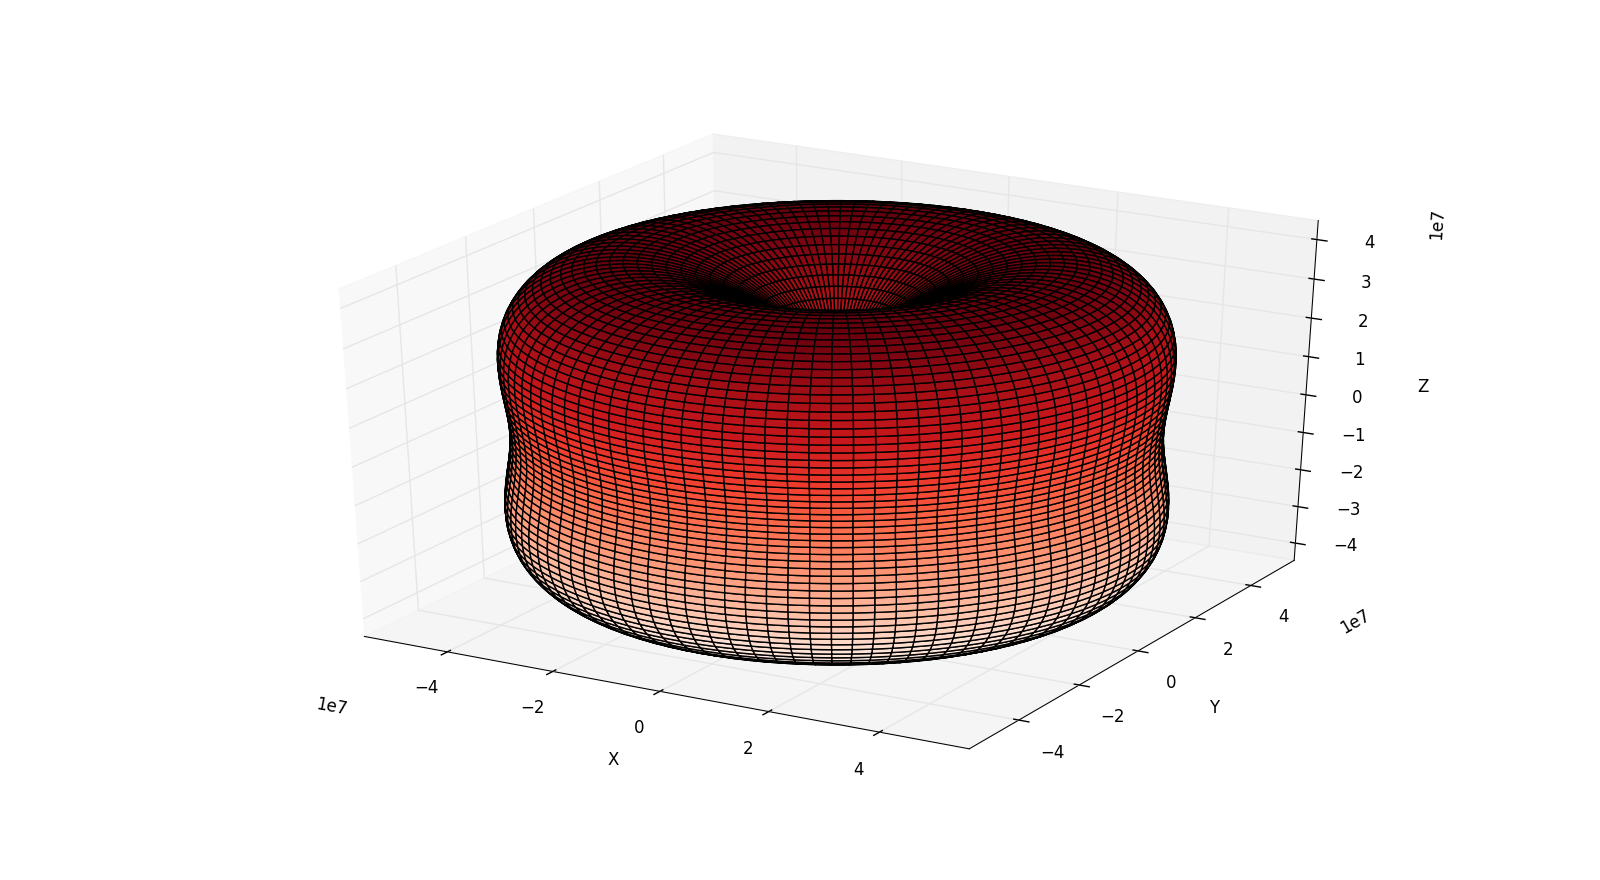
\includegraphics[height=0.7\textheight]{near_kr_0_1_1.png}
    \caption*{\tiny{kr=0.1}}
  \end{figure}
\end{frame}
% frame_
\begin{frame}
  \frametitle{Patten of Near-Field Region}
  \begin{figure}
    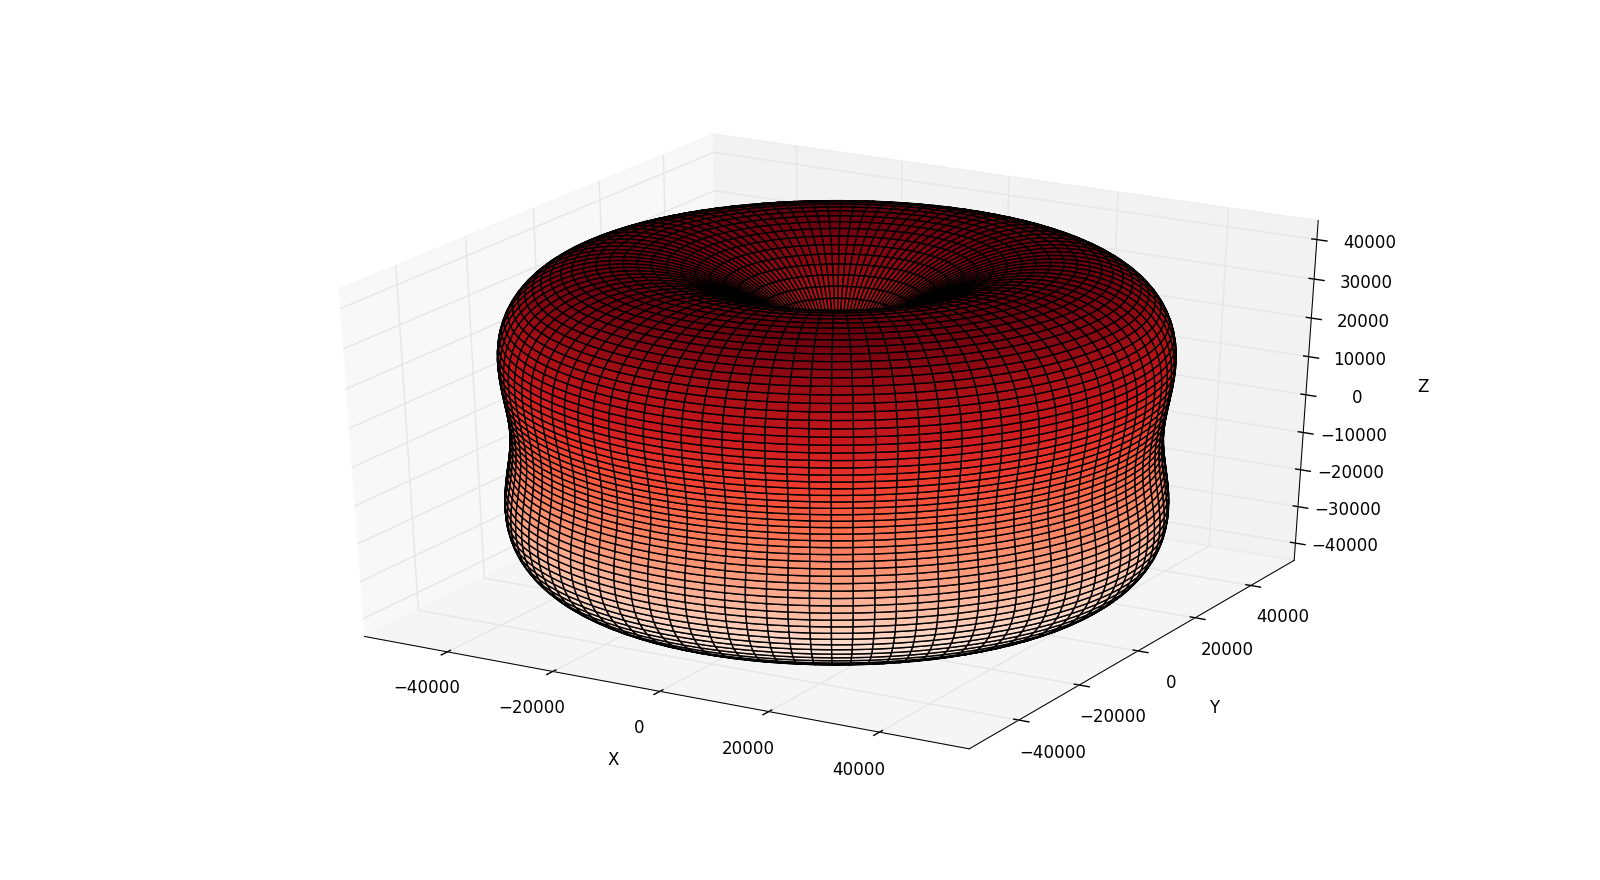
\includegraphics[height=0.7\textheight]{near_kr_1_1.png}
    \caption*{\tiny{kr=1}}
  \end{figure}
\end{frame}


%% Inter
% frame_
\begin{frame}
  \frametitle{Patten of Intermediate-Field Region}
  \begin{block}{~}
  \begin{equation}
    \left.
      \begin{array}{l}
        E_r \simeq {\eta}\frac{I_0le^{-jkr}}{1\pi r^1}\cos{\theta}\\\\
        E_{\theta} \simeq j{\eta}\frac{kI_0le^{-jkr}}{4\pi r}\sin{\theta}\\\\
        E_{\phi}=H_r=H_{\theta}=0\\\\
        H_{\phi}\simeq j\frac{kI_0le^{-jkr}}{4\pi r}\sin{\theta}
      \end{array}
    \right\} kr>1 
  \end{equation}
\end{block}
\end{frame}
% frame_
\begin{frame}
  \frametitle{Patten of Intermediate-Field Region}
  \begin{figure}
    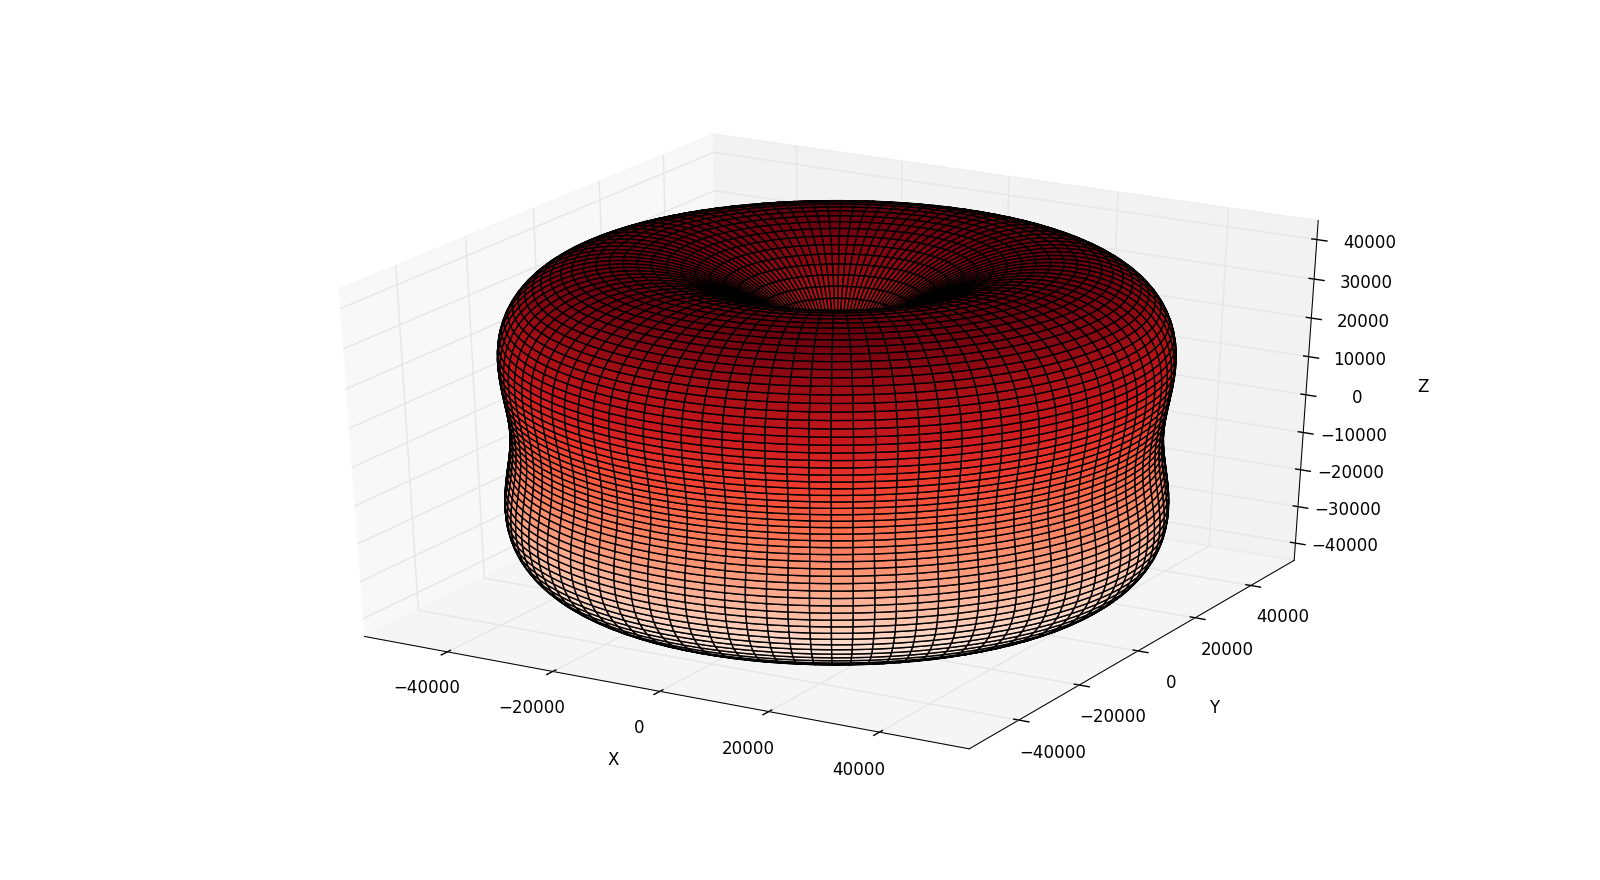
\includegraphics[height=0.7\textheight]{inter_kr_1_1.png}
    \caption*{\tiny{kr=1}}
  \end{figure}
\end{frame}
% frame_
\begin{frame}
  \frametitle{Patten of Intermediate-Field Region}
  \begin{figure}
    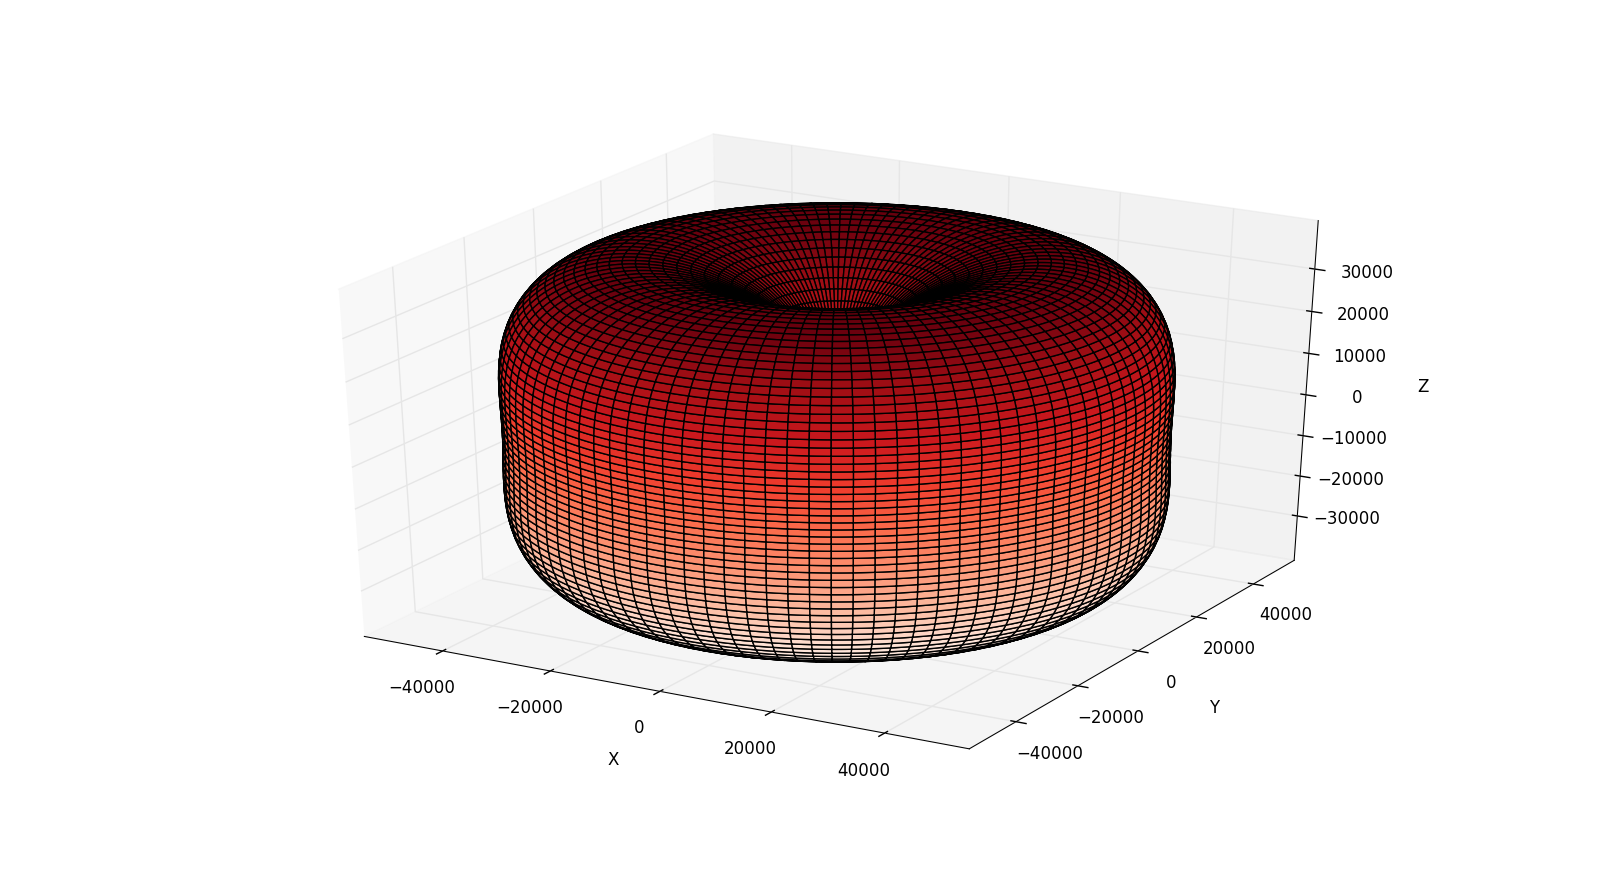
\includegraphics[height=0.7\textheight]{inter_kr_1_1_1.png}
    \caption*{\tiny{kr=1.1}}
  \end{figure}
\end{frame}
% frame_
\begin{frame}
  \frametitle{Patten of Intermediate-Field Region}
  \begin{figure}
    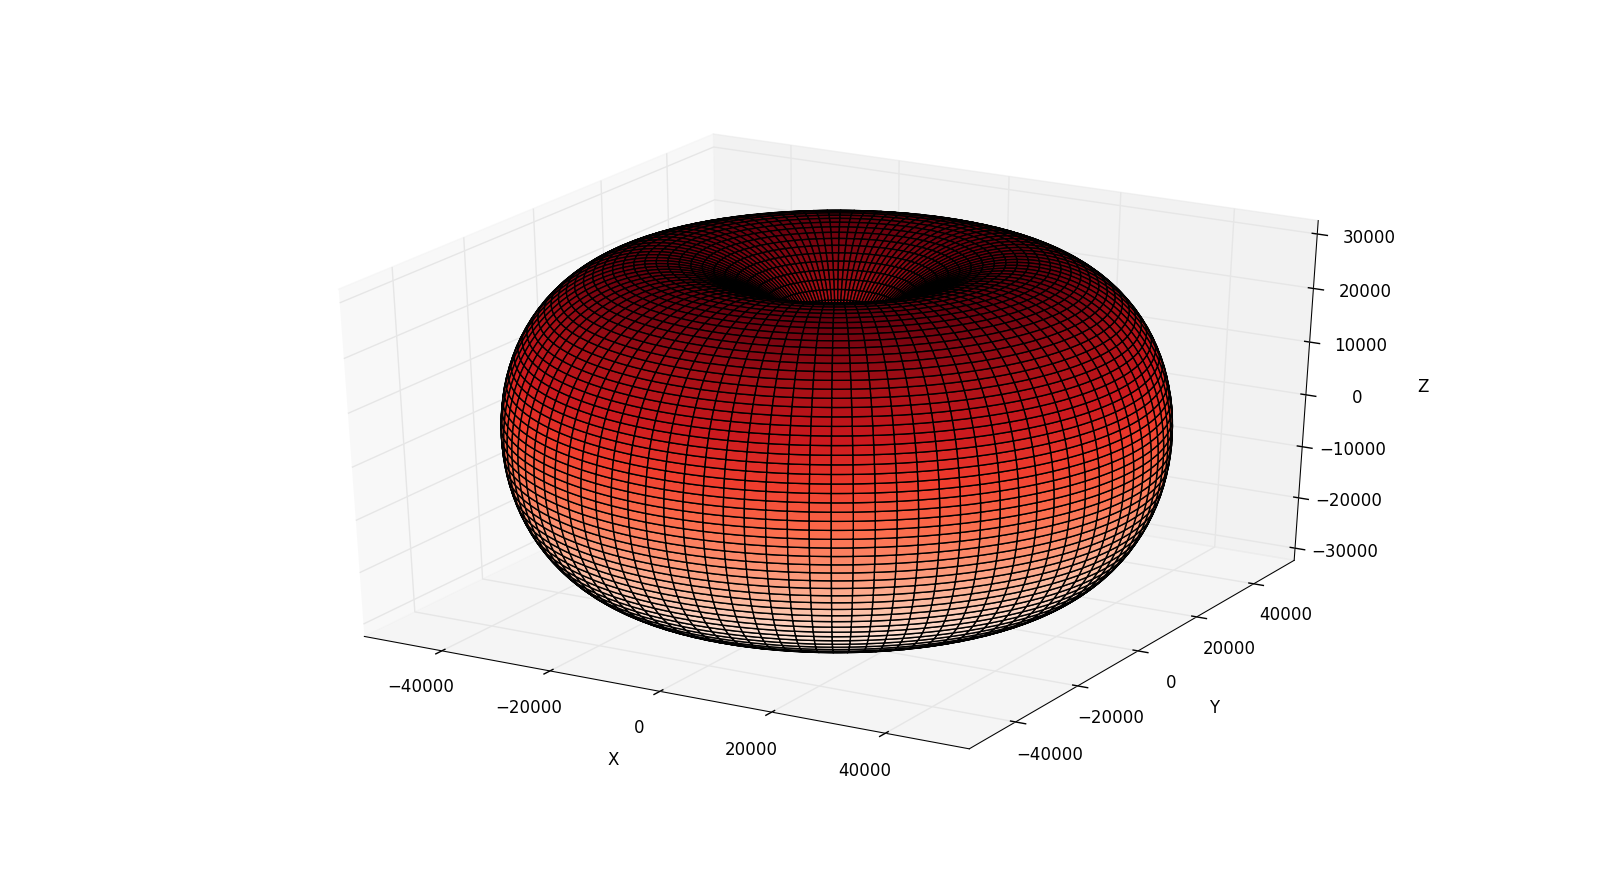
\includegraphics[height=0.7\textheight]{inter_kr_1_5_1.png}
    \caption*{\tiny{kr=1.5}}
  \end{figure}
\end{frame}
% frame_
\begin{frame}
  \frametitle{Patten of Intermediate-Field Region}
  \begin{figure}
    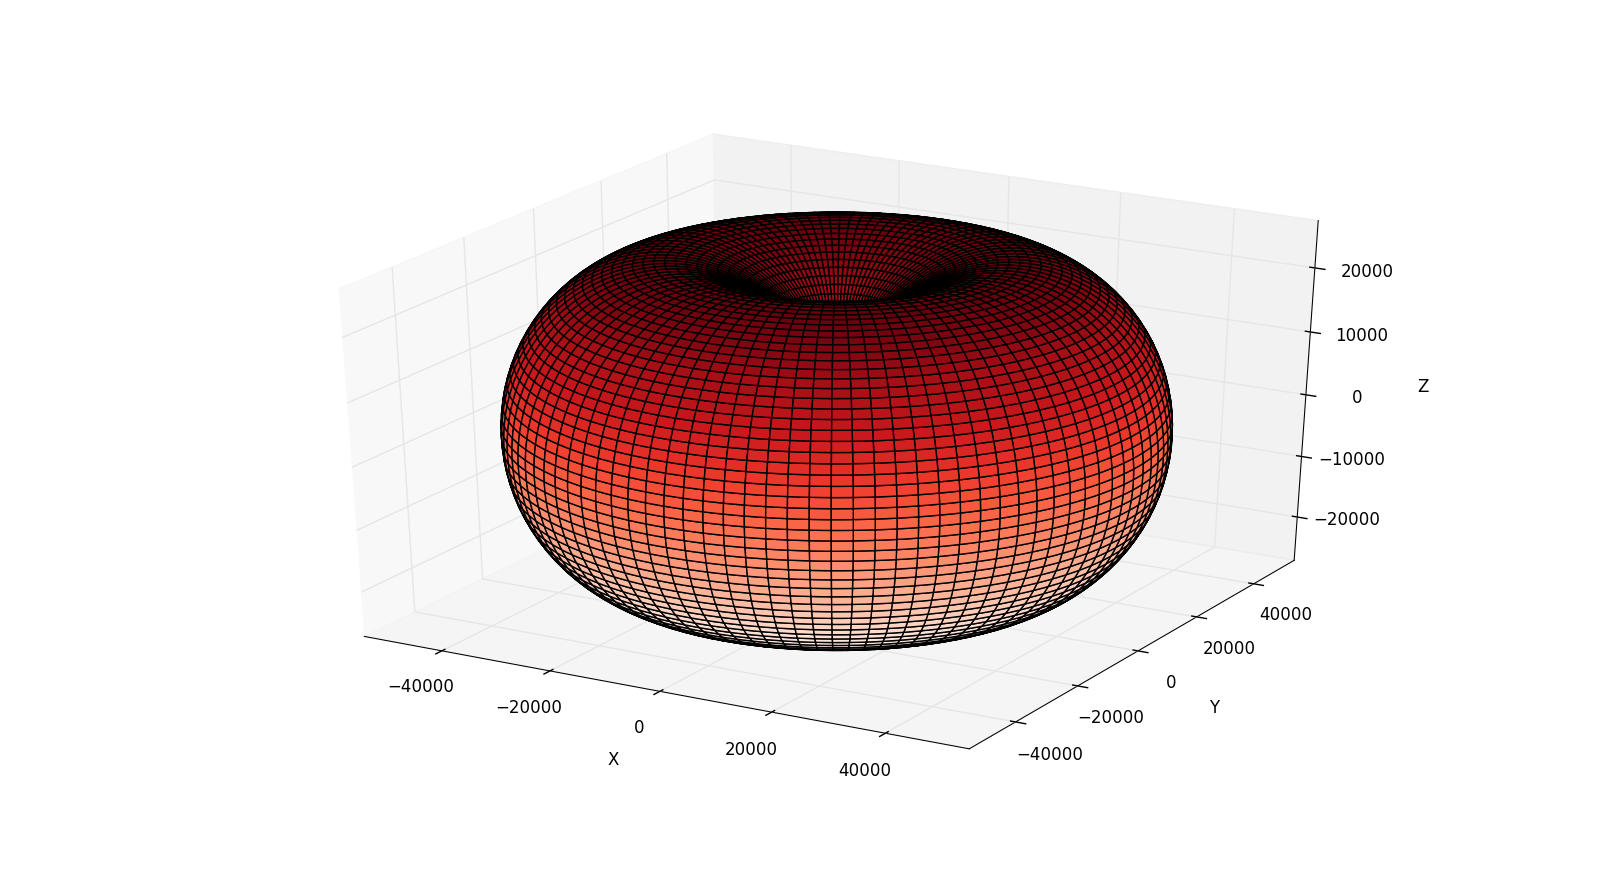
\includegraphics[height=0.7\textheight]{inter_kr_2_1.png}
    \caption*{\tiny{kr=2}}
  \end{figure}
\end{frame}
% frame_
\begin{frame}
  \frametitle{Patten of Intermediate-Field Region}
  \begin{figure}
    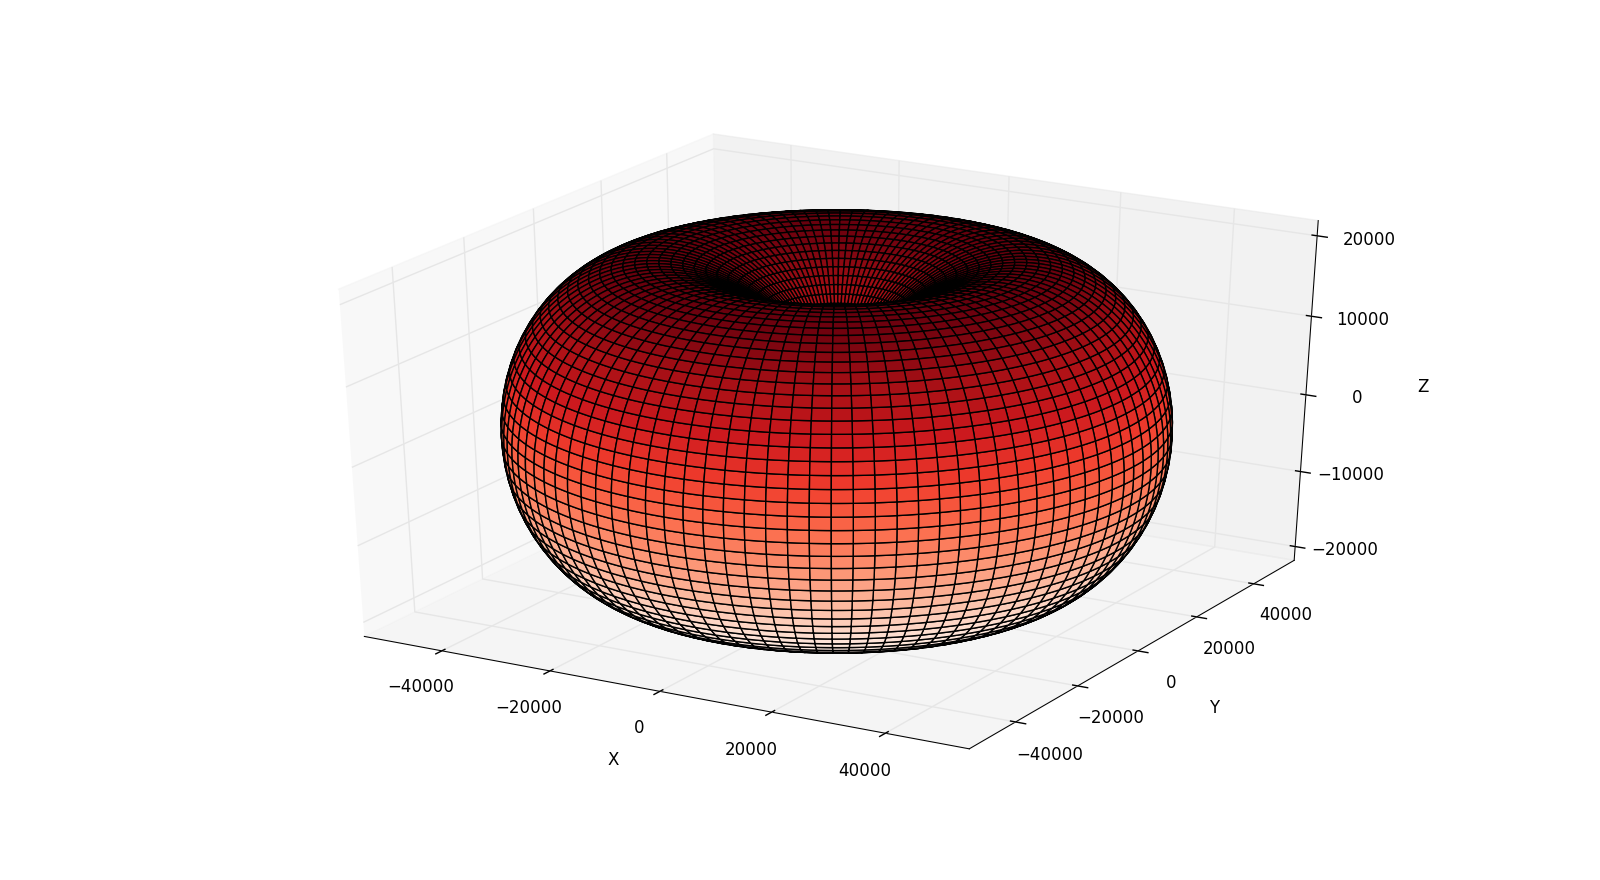
\includegraphics[height=0.7\textheight]{inter_kr_5_1.png}
    \caption*{\tiny{kr=5}}
  \end{figure}
\end{frame}



%% far
% frame_
\begin{frame}
  \frametitle{Far-Field Region}
  \begin{block}{~}
  \begin{equation}
    \left.
      \begin{array}{l}
        E_{\theta} \simeq j{\eta}k\frac{I_0le^{-jkr}}{4\pi r}\sin{\theta}\\\\
        E_r=E_{\phi}=H_r=H_{\theta}=0\\\\
        H_{\phi}\simeq j\frac{kI_0le^{-jkr}}{4\pi r}\sin{\theta}
      \end{array}
    \right\} kr\gg 1
  \end{equation}
  \end{block}
\end{frame}
% frame_
\begin{frame}
  \frametitle{Patten of Far-Field Region}
%  \framesubtitle{kr=0.01}
  \begin{figure}
    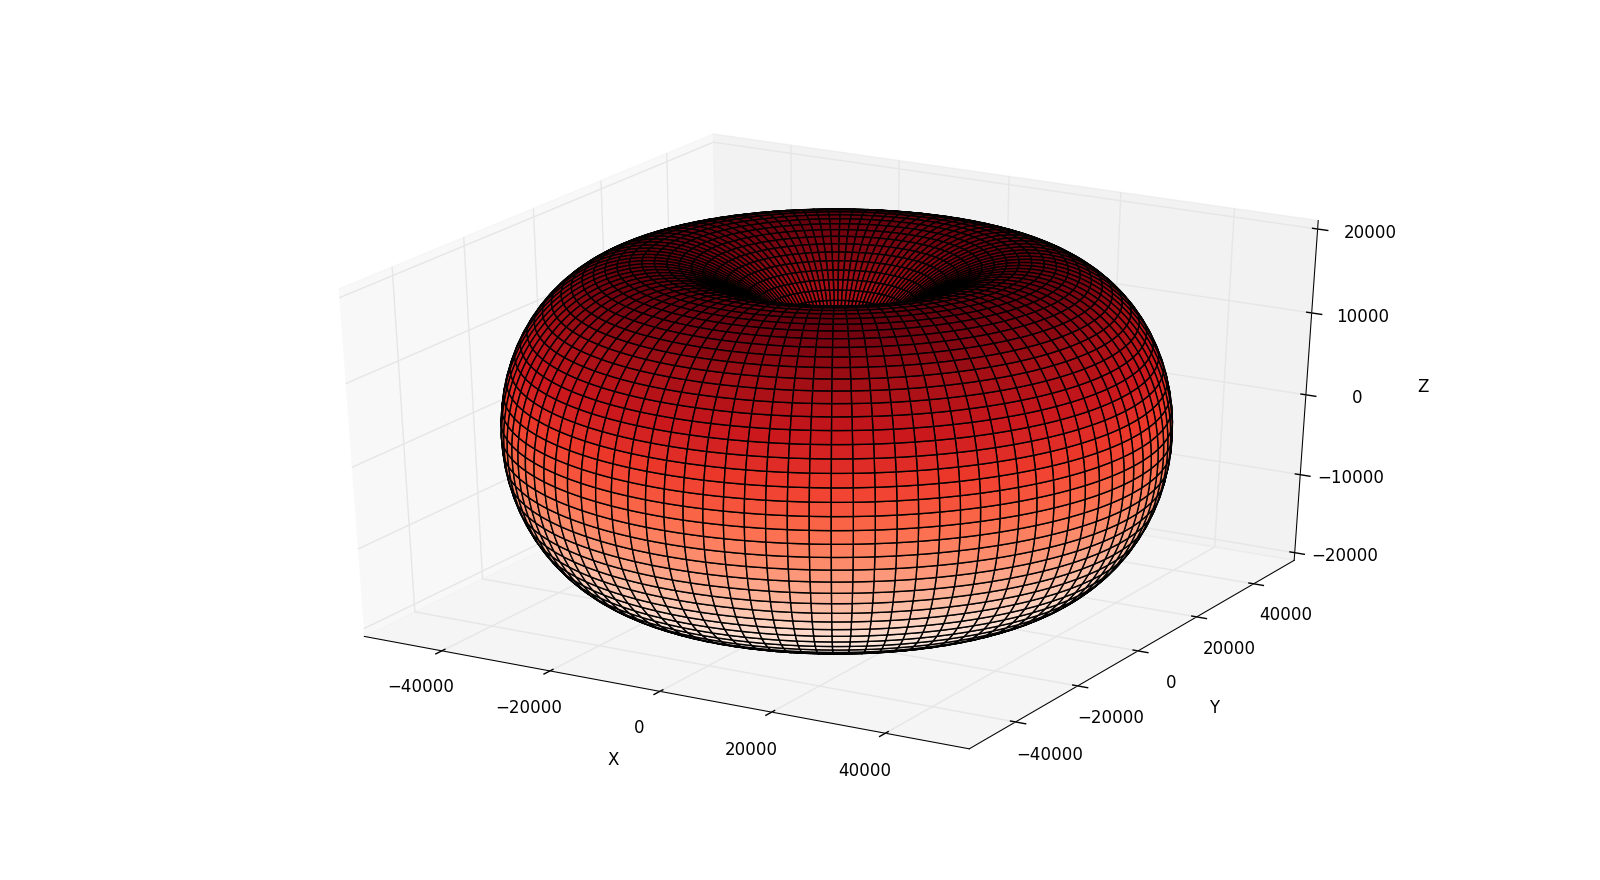
\includegraphics[height=0.7\textheight]{far_kr_10_1.png}
    \caption*{\tiny{kr=10}}
  \end{figure}
\end{frame}
\begin{frame}
  \frametitle{Patten of Far-Field Region}
%  \framesubtitle{kr=0.01}
  \begin{figure}
    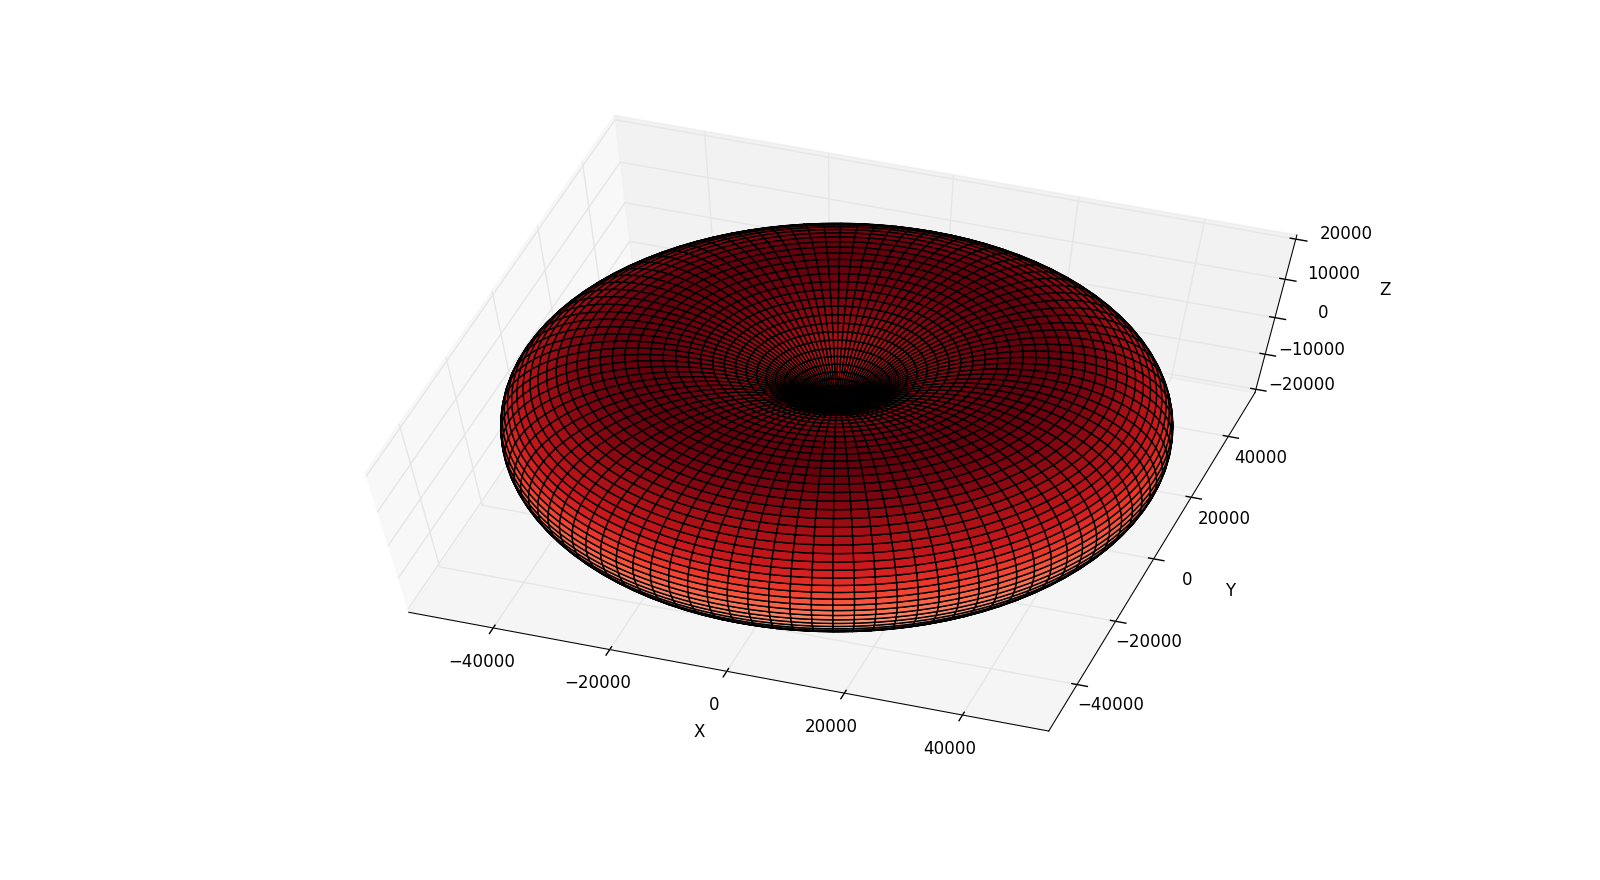
\includegraphics[height=0.7\textheight]{far_kr_10_2.png}
    \caption*{\tiny{kr=10}}
  \end{figure}
\end{frame}
\begin{frame}
  \frametitle{Patten of Far-Field Region}
%  \framesubtitle{kr=0.01}
  \begin{figure}
    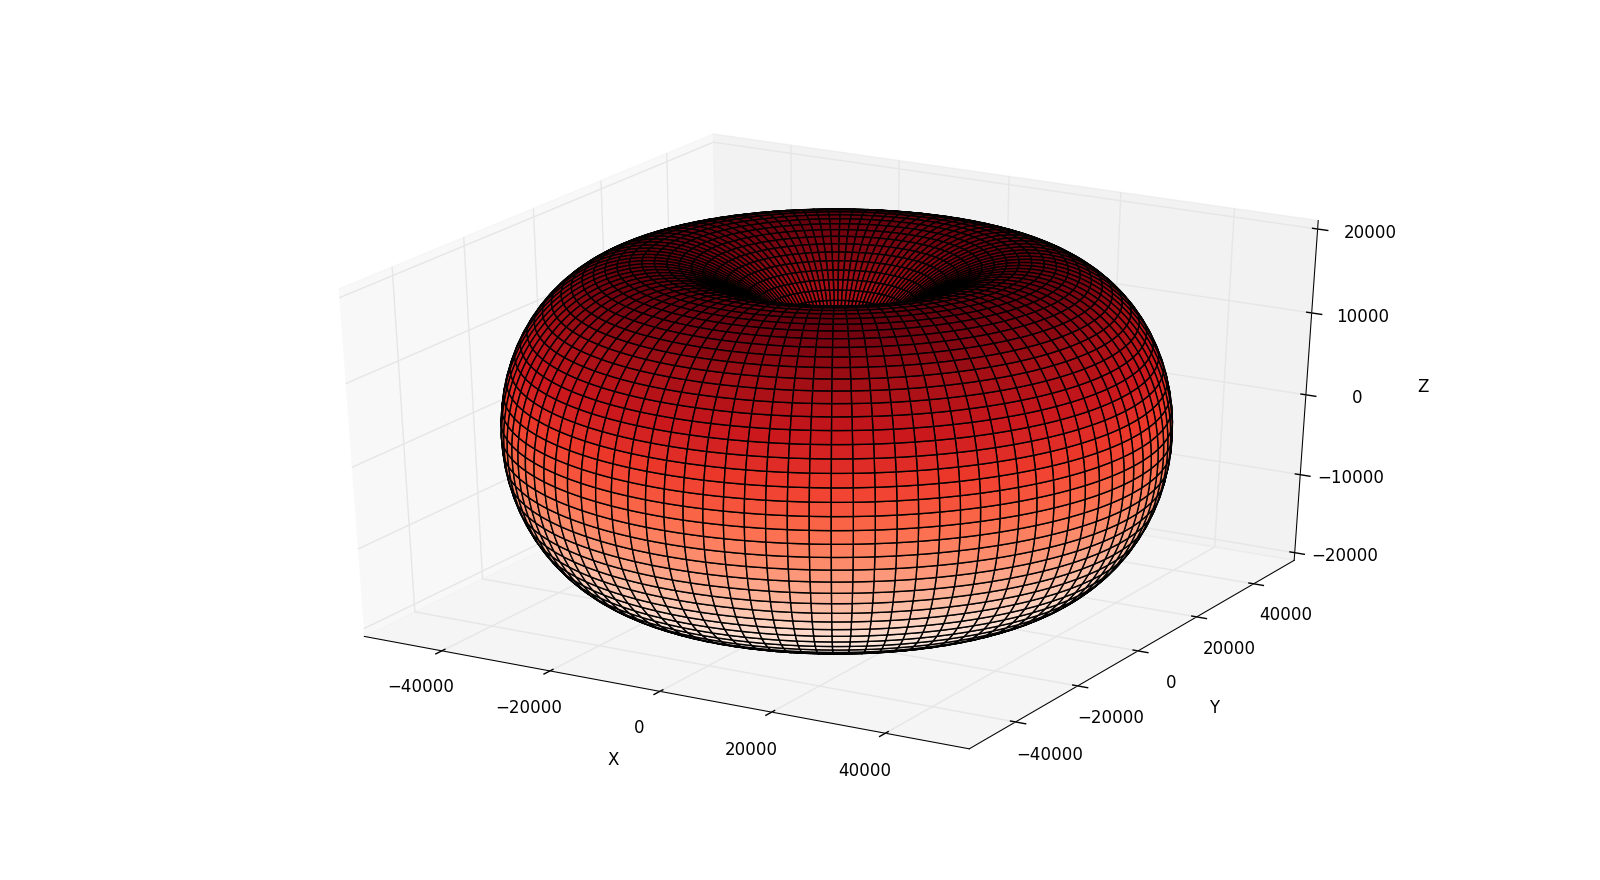
\includegraphics[height=0.7\textheight]{far_kr_100_1.png}
    \caption*{\tiny{kr=100}}
  \end{figure}
\end{frame}
\begin{frame}
  \frametitle{Patten of Far-Field Region}
%  \framesubtitle{kr=0.01}
  \begin{figure}
    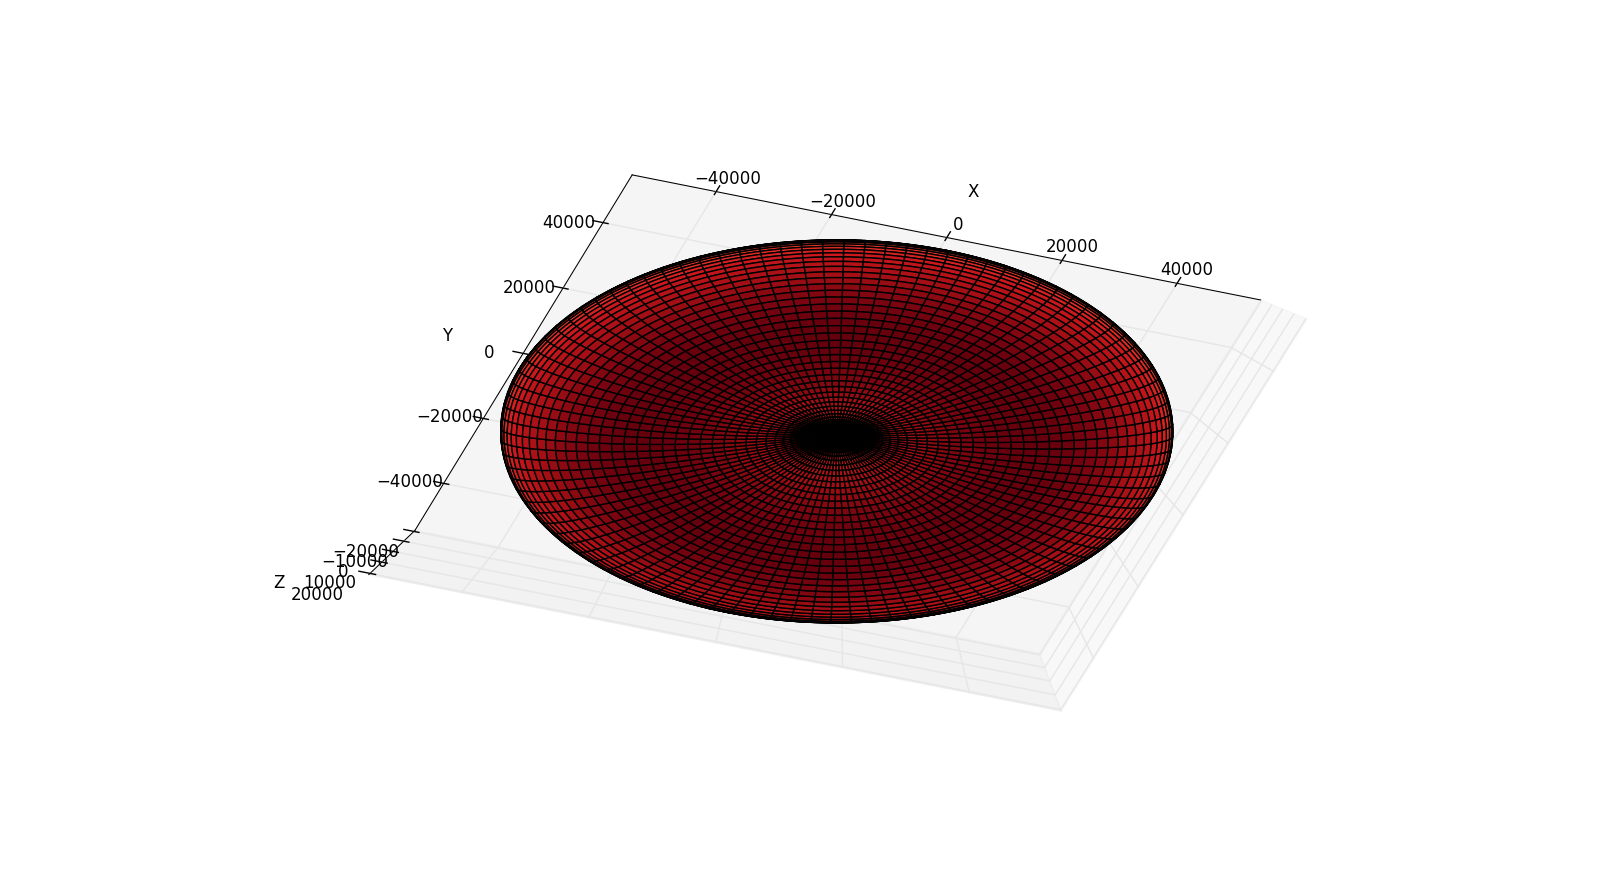
\includegraphics[height=0.7\textheight]{far_kr_100_2.png}
    \caption*{\tiny{kr=100}}
  \end{figure}
\end{frame}
% frame_
\begin{frame}
  \frametitle{Patten of Far-Field Region}
  \begin{figure}
    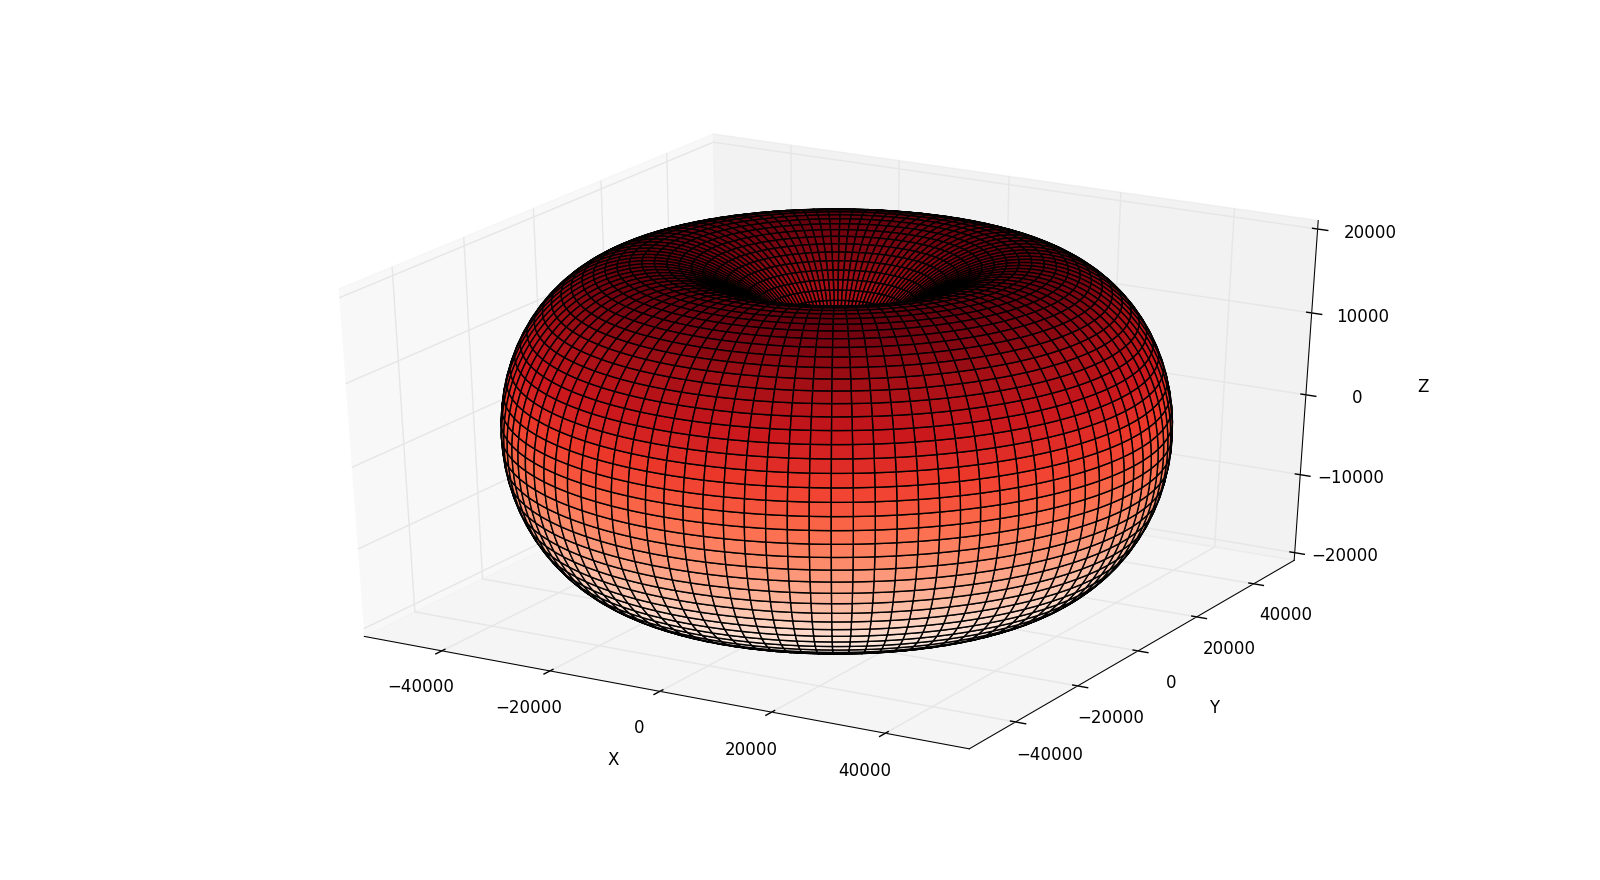
\includegraphics[height=0.7\textheight]{far_kr_10000_1.png}
    \caption*{\tiny{kr=10000}}
  \end{figure}
\end{frame}

\end{document}
